\chapter{Experiments}

In this chapter we give the results of our experiments on the SBM.  
\section{Spectral Clustering on the Bethe Hessian for the SBM}
\begin{definition}The 
\textit{Bethe Hessian} is a one parameter perturbation of the unnormalized graph Laplacian.  Let $D$ be the diagonal matrix of degree of graph $G$ and $\mathbb{I}$ be the identity matrix in $n$ dimensions (where $G$ has $n$ vertices).  We define the Bethe Hessian as a matrix that depends on $r \in \mathbb{R}$ as  $$BH(r) := (r^2-1)\mathbb{I} - rA +D.$$
\end{definition}

Saade et al. showed in \cite{AFL} that the Bethe Hessian was a competitive matrix to do spectral clustering on when close to the information theoretic threshold of detection of the SBM.  It has the benefit of being easily computed from the adjacency matrix. Recall that the information theoretic threshold for SBM($n, a/n, b/n)$ occurs for bounded degree graphs $G$ when $(a-b)^2 = 2(a+b)$.  When $(a-b)^2 > 2(a+b)$ we can recover the communities, when $(a-b)^2 < 2(a+b)$ we cannot.  Saade et al. did an experiment to compare bounded degree graphs with average degree 3, and compared various spectral methods, as well as belief propagation with spectral clustering on the Bethe Hessian. The best $r$ to use for the Bethe Hessian was motivated by results in statistical physics. It was empirically shown to give good accuracy for $r$ equal to the root of the average degree of the graph in the case of the SBM, but in general requires one to solve an eigenproblem on the graph zeta function.  See \cite{AFL} for details. 

\begin{figure}[h]
  \begin{center}
  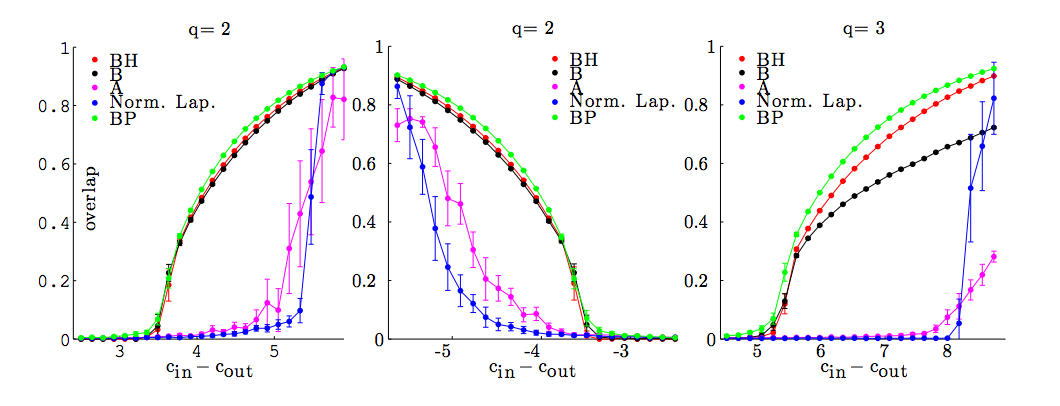
\includegraphics[scale=0.4]{BH_SBM.png}
  \caption{Spectral clustering with the Bethe Hessian compared to other popular methods that work at the limit of clustering detectability. Average degree of all SBM graphs is 3 (extremely sparse regime). This graph of results is taken from \cite{AFL} and shows the optimality of using BH, allowing spectral methods to be efficient even at the informational theoretic boundary of this problem.}
  \end{center}
\end{figure}

Our first experiment is to see if the GNN can learn the optimal scalar $r$ such that spectral clustering with $BH(r)$ becomes informative. Of course, since $r$ is a scalar, it is more efficient to brute force search for the solution rather than use gradient descent. However this preliminary experiment is meant to show that gradient descent can retrieve the optimal $r$ given the GNN architecture's ability to approximate the power method in order to find the eigenvectors of $BH(r)$.  

To be clear, the experimental task is as follows.

\begin{itemize}
    \item Input: Adjacency matrices A (instantiated from specific $SBM(n,a/n, b/n)$). 
    \item The parameter to be learned via gradient descent is $r$ of $BH(r)$. 
    \item Output: A community assignment of vertices : $F : V \rightarrow \{0,1\}$. 
\end{itemize}

The model was able to decrease loss, converge and get close to the theoretically verified optimal $r$. 

\begin{figure}
\begin{center}
  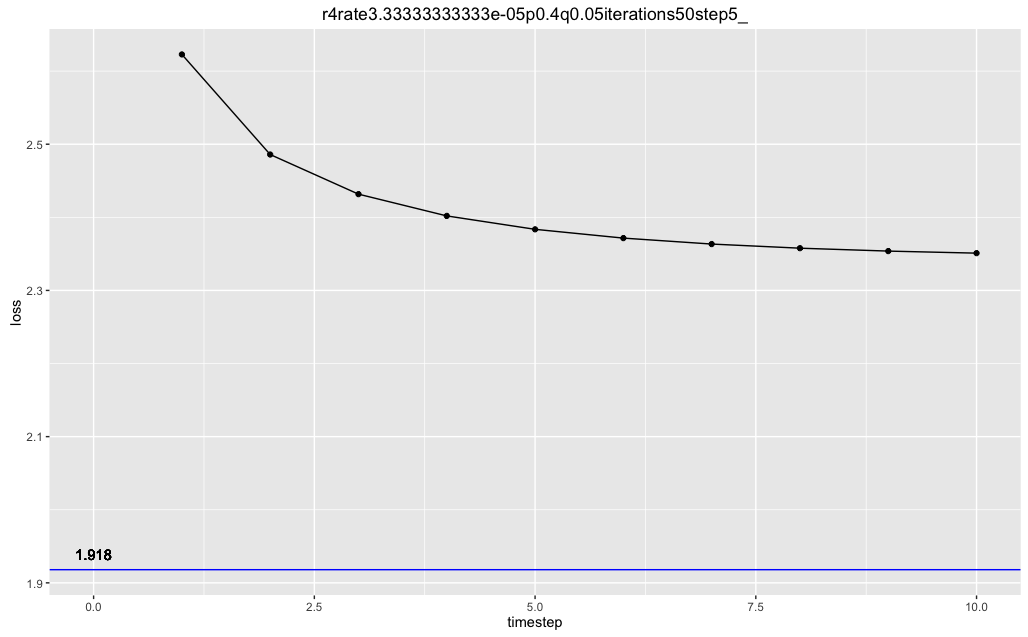
\includegraphics[width=0.8\textwidth]{50steps.png}
   \caption{$p=0.4, q=0.05$, 50 iterations}
  \label{fig:GNN_BH}
 \end{center}
\end{figure}

\begin{figure}
\begin{center}
  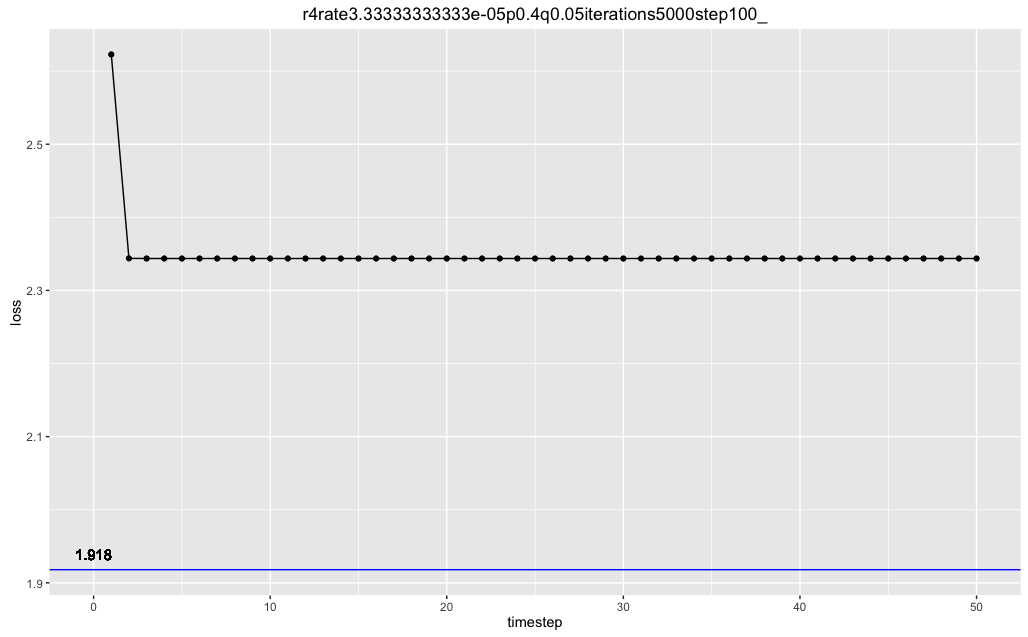
\includegraphics[width=0.8\textwidth]{500steps.png}
   \caption{$p=0.4, q=0.05$, 5000 iterations}
  \label{fig:GNN_BH_1}
 \end{center}
\end{figure}

\begin{figure}[H]
\begin{center}
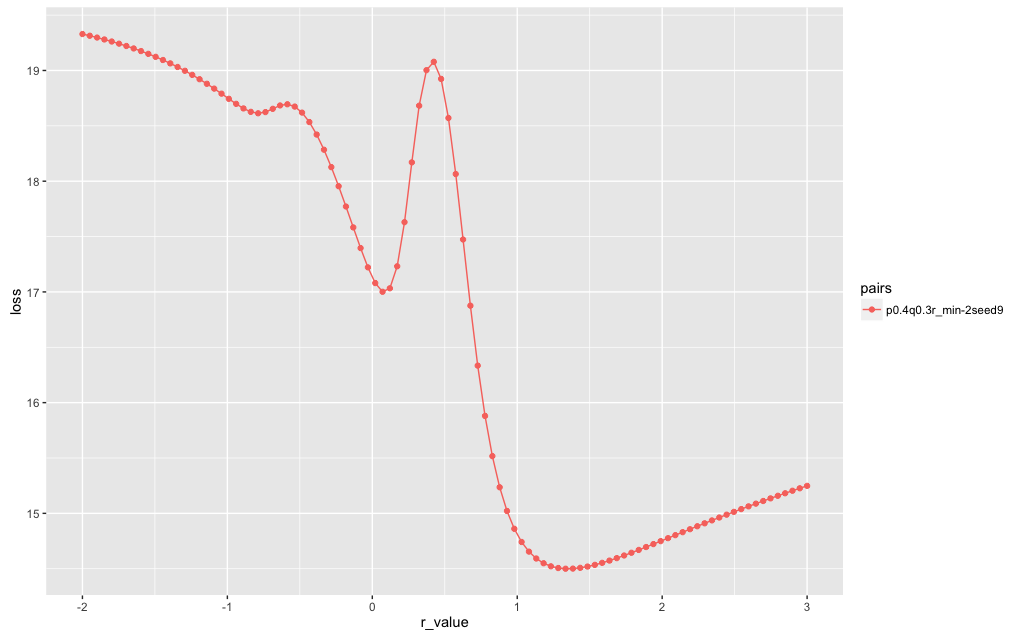
\includegraphics[scale=0.4]{loss_surface_1.png}
\caption{Bethe Hessian loss surface 1.}
 \end{center}
\end{figure}

\begin{figure}[H]
\begin{center}
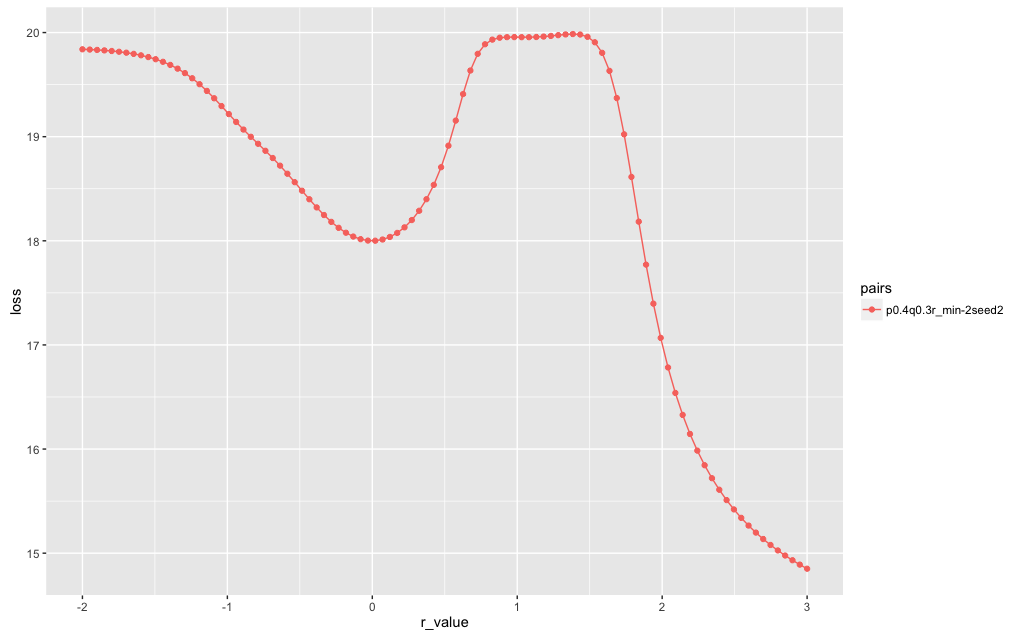
\includegraphics[scale=0.4]{loss_surface_2.png}
\caption{Bethe Hessian loss surface 2.}
 \end{center}
\end{figure}

\begin{figure}[H]
\begin{center}
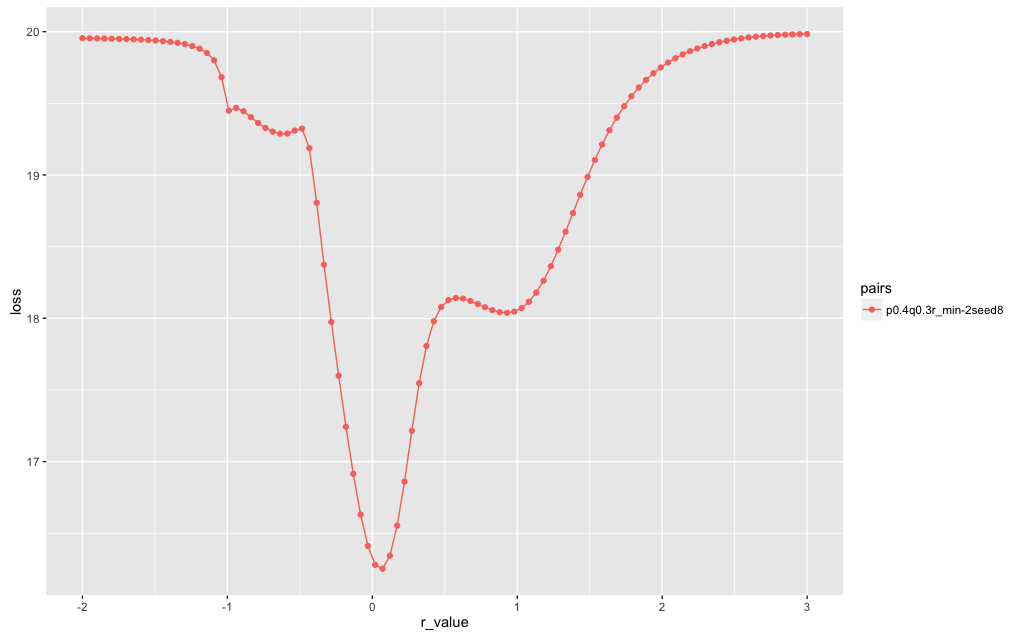
\includegraphics[scale=0.4]{loss_surface_3.png}
\caption{Bethe Hessian loss surface 3.}
 \end{center}
\end{figure}

\begin{figure}[H]
\begin{center}
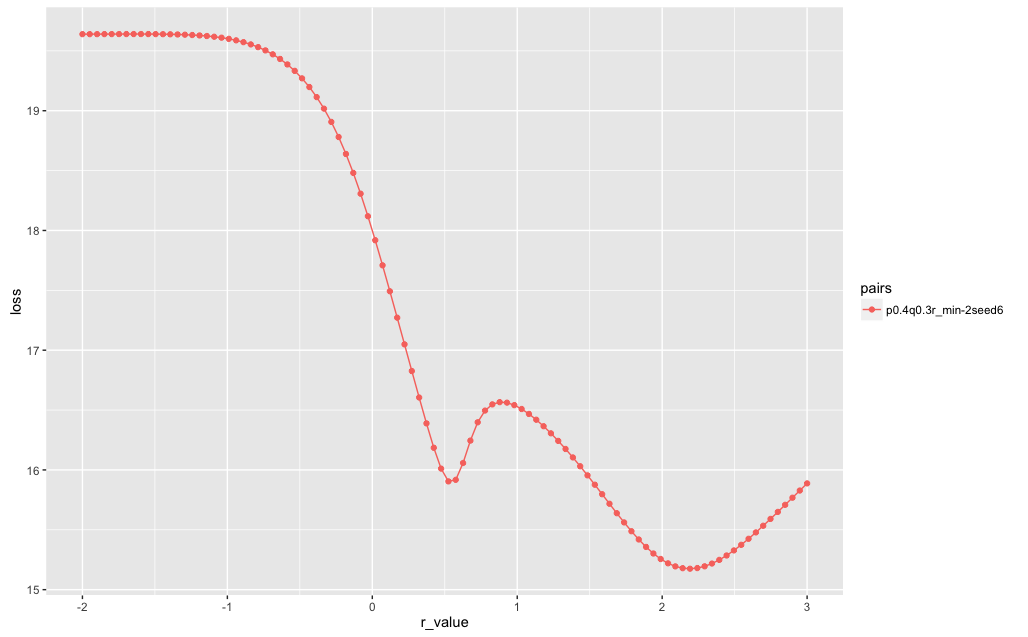
\includegraphics[scale=0.4]{loss_surface_4.png}
\caption{Bethe Hessian loss surface 4.}
 \end{center}
\end{figure}
 
Learning a one dimensional parameter $r$ is a proof of concept.  It forces an artificially hard bottleneck on our gradient optimization problem since the one dimensional loss surface is clearly non-convex and contains lots of non-optimal local optima. The optimization landscape is also highly varied depending on the instantiation of SBM.  What this section serves to confirm empirically is that the power method for a very specific matrix is within the expressive power of the GNN and that gradient descent can successfully find the scalar that best optimizes the spectral signal in that case. 

\newpage

\section{GNN Performance Near Information Theoretic Threshold}
\begin{figure}[H]
\begin{center}
  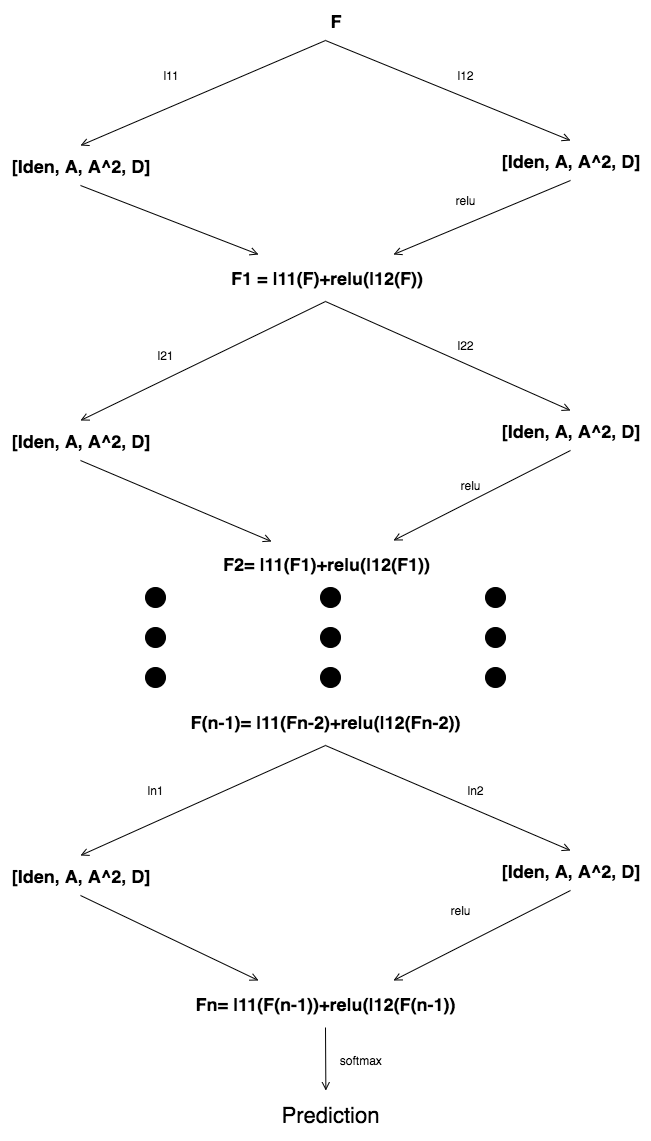
\includegraphics[scale=0.47]{GNN_SBM.png}
  \caption{Graph Neural Network architecture for information theoretic boundary for community detection.}
  \label{fig:GNN}
\end{center}
\end{figure}

For the main experiment, we consider a GNN with the structure shown in figure \ref{fig:GNN}.

In figure \ref{fig:GNN}, our input is $F\in \mathbb{R}^{n \times k}$ where $n$ is the number of nodes and $k$ is the dimension of the signal.  In a clustering problem, $k$ can be the number of communities we want to detect, where $\mathbb{R}^{n\times k}$ is a one-hot encoding of the clustering (an encoding where a categorical vector with $k$ categories is replaced with $k$ column vectors where each entry is 1 if it is in the category and 0 otherwise). At each layer, the input signal $F$ is transformed via a convolution applied to the following array of operators:  $[Iden, A, A^2, D]$.  $Iden$ is the identity matrix the size of the graph adjacency matrix.  $A$ is the graph adjacency matrix.  And $D$ is a matrix with the degree of each vertex on its diagonal (and zeros everywhere else). 

In the language of operators introduced in the previous section, each layer we have the following $$ F_1^{n+1} = \eta(Iden \cdot F^n, A \cdot F^n, A^2 \cdot F^n, D \cdot F^n)$$ and $$ F_2^{n+1} = Relu \circ \eta(Iden \cdot F^n, A \cdot F^n, A^2 \cdot F^n, D \cdot F^n)$$ and $$ F^{n+1} = F_1^{n+1}+F_2^{n+2}$$
where $\eta$ is a spatial convolution and $Relu(x) := max(0, x)$ (Relu applied to vectors is just Relu applied elementwise).  For our network applied to the SBM, we used 16 channels per layer, and 20 layers for a 1000 node graph. In the first layer each layer we apply a $k \times 4$ convolution to each of the 16 output channels.  The number of communities is given by $k$.  The final layer outputs to $k$ channels, to correspond to the $k$ dimensional one hot encoding of the community labels. We furthermore normalize and center after each layer for stability.  

The accuracy measure is given by the overlap. 
\begin{definition}The \textit{Overlap} between a true community label $g: V \rightarrow V$ where $g(u) := g_u$, and the predicted community label $\bar{g}:V \rightarrow V$ where $\bar{g}(u) := \bar{g_u}$, is given by
$$ \frac{\big(\frac{1}{n}\sum_u \delta_{g_u, \bar{g_u}} - \frac{1}{k}\big)}{(1-\frac{1}{k})}$$

where $\delta$ is the Kronecker delta function.  
\end{definition}

The clustering overlap performance of the GNN in the information theoretic threshold for the SBM in both assortative and dissortative regime are in graphs \ref{fig:ass}, \ref{fig:diss} and \ref{fig:k3}.  The regime is extremely sparse, where $n =1000$ and the average degree is $3$.  The x-axis is gives the difference in average degrees of the subgraph induced by nodes in the same community and between nodes in different communities: $c_{in} - c_{out}$.  Another way to interpret $c_in$ and $c_out$ is via $c_in/n = p$ and $c_out/n = q$.  The clustering problem becomes easier as $|c_in-c_out|$ grows.  

\begin{figure}[H]
\begin{center}
  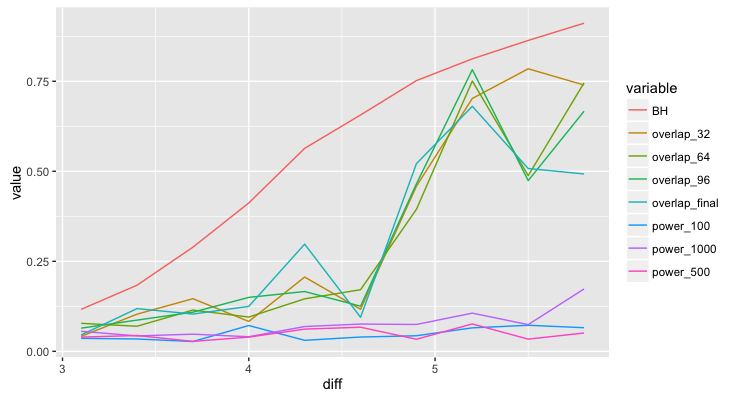
\includegraphics[scale=0.55]{asso.png}
  \caption{Performance of GNN against BH baseline for n=1000 at information theoretic threshold with assortative communities.}
  \label{fig:ass}
\end{center}
\end{figure}

\begin{figure}[H]
\begin{center}
  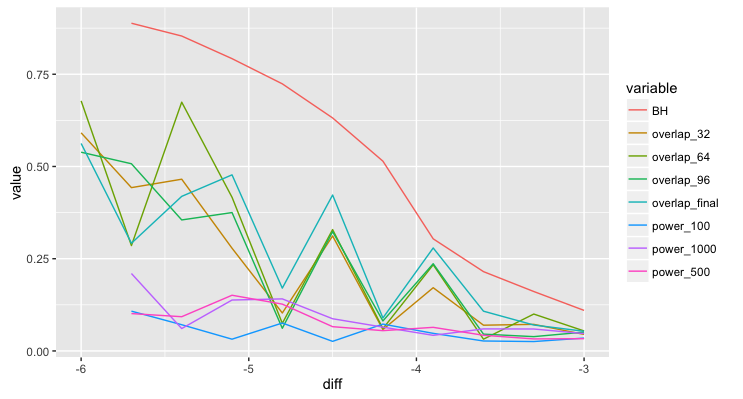
\includegraphics[scale=0.55]{diss.png}
  \caption{Performance of GNN against BH baseline for n=1000 at information theoretic threshold with dissortative communities.}
  \label{fig:diss}
\end{center}
\end{figure}

\begin{figure}[H]
\begin{center}
  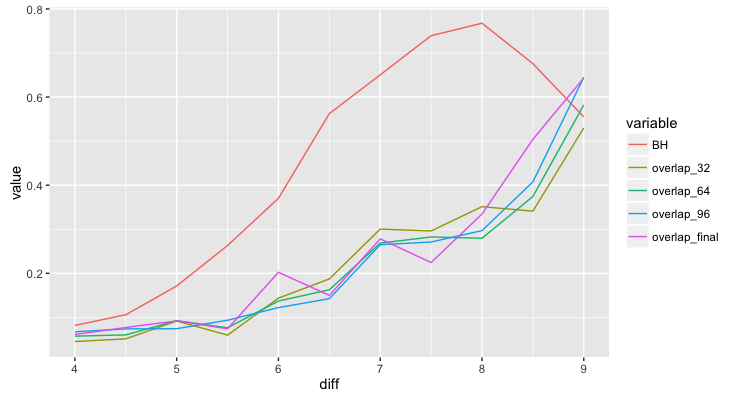
\includegraphics[scale=0.55]{k3.png}
  \caption{Performance of GNN against BH baseline for n=1000 at information theoretic threshold with 3 communities.}
  \label{fig:k3}
\end{center}
\end{figure}


\section{Future Directions}

We have shown the success of the graph neural network on even the most extreme cases of the SBM.  Current extensions of this work is being done by the author and Joan Bruna to apply to real datasets in the area of community detection in social networks, as well as more diverse problems that involve signals on graphs, including ranking, entity detection in databases and protein interaction detection. 
